\section{The Model}
This section will showcase the model made to express the design from \myref{cha:Design}.
For simplicity the introduction of the model in this chapter has split the model into two parts, an initializing phase and the main loop.
The complete model can be seen in \myref{app:UPPAAL} along with the code for the global and local declarations, including the functions used throughout the model.

The first part to be shown will be the initialization, which can be seen on \myref{fig:UPPAAL_Intitialization}

\begin{figure}
  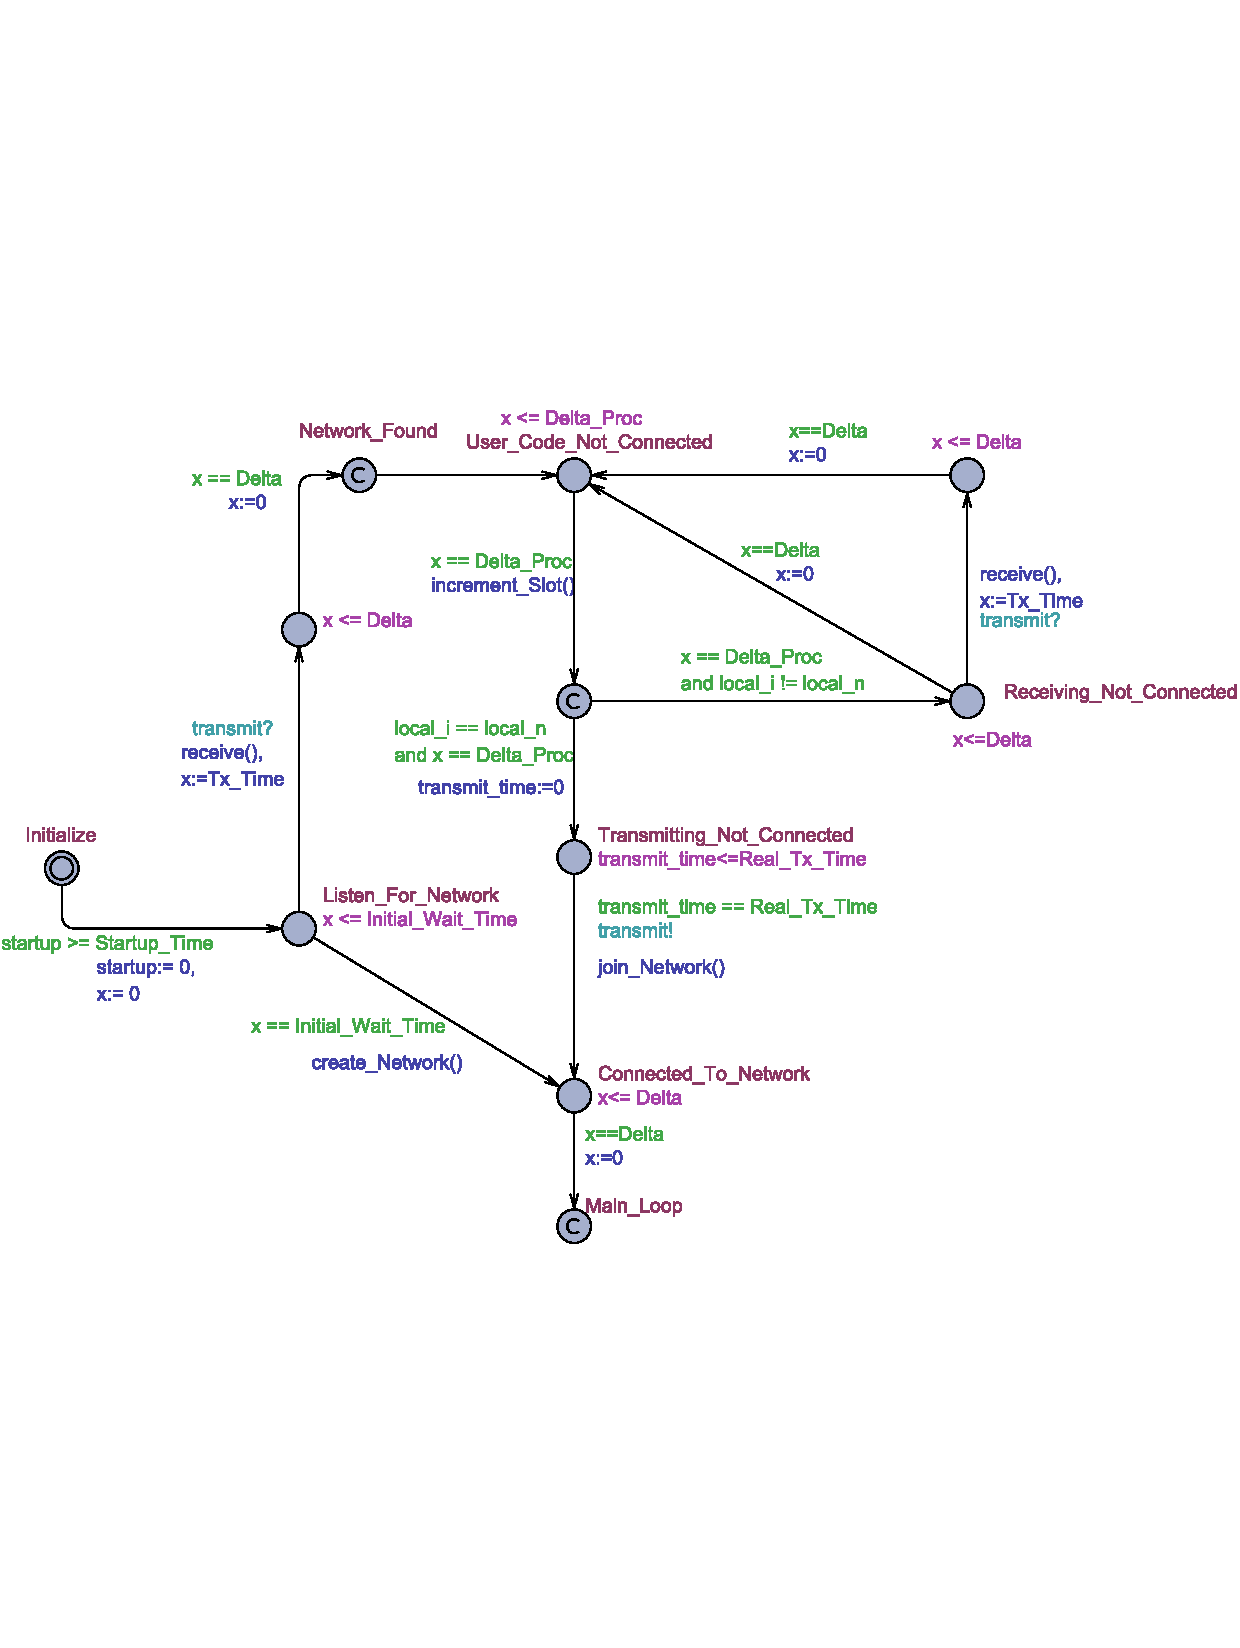
\includegraphics[width=1\textwidth]{Figures/Model/Device_Connecting.pdf} 
\caption{UPPAAL Model showing how the devices initialize.}
\label{fig:UPPAAL_Intitialization}
\end{figure}

The initial state has a clock \texttt{startup}, which makes sure that only one of the devices will be leaving the initial state at the same time.
When one of the devices leave this state the clock will reset, and another will leave the state when the \texttt{startup} once again reaches the desired time.
It has to be mentioned that this wait time for startup has to be increased with the number of devices connecting to the network. 
When the frame is larger, this startup wait time has to be increased to make sure that only one device will try to connect in the empty slot.
With the current values creating a network with six devices is doable.
While the other devices are waiting to be released, the device which was the first to leave will listen for a network, as there is obviously no network yet the device will fire the edge towards the \texttt{Creating\_Network} state.
The device will setup the initial values for the network, change its boolean \texttt{Connected} to true, and start the main loop.
When the next device leaves the initial stage, it will when it is listening for a network be successful as a network has just been created, which means that the device will move towards the committed state \texttt{Network\_Found} and reset the clock \texttt{x} to zero.
This state is committed as its purpose is simply context switching between receiving and performing user code.
When it has just received a transmission, the device which just transmitted will according to \myref{cha:Design} be performing user code, and so should the device trying to connect.
When \texttt{x} is equal to \texttt{Delta\_Com}, which is the time given to a device to perform user code, the device will change to the state \texttt{Network\_Found} once again.
In this state when \texttt{x} is not zero, the device checks whether \texttt{i}, which is the current time-slot, is the empty-time slot, if it is the device will transmit, and ultimately connect to the network, increasing the number of time-slots in the network according to the specifications from \myref{cha:Design}.
If the empty slot was not the current time-slot, the device will instead go to the state \texttt{Receiving\_Not\_Connected} where it will receive the other devices' transmissions, and once again reset \texttt{x} to zero, and perform user code, until eventually the empty-slot occurs, where it will connect to the network.

The committed state \texttt{Connected\_To\_Network} has 3 edge leaving it, one for receiving, one for transmitting, and one of executing user code.
The model can be seen on \myref{fig:UPPAAL_Connected}.

\begin{figure}
  
\includegraphics[width=1\textwidth]{Figures/Model/Device_Connected.pdf} 
\caption{UPPAAL Model showing the devices' main loop.}
\label{fig:UPPAAL_Connected}
\end{figure}

It works the roughly the same as the state \texttt{Network\_Found}, except the guard checking whether it is the empty time-slot instead checks whether it is the device's time-slot.
Another change is when the device is in the state \texttt{Receiving}, if nothing has been transmitted and the clock \texttt{x} is equal to \texttt{Delta} the device will go increment its \texttt{i\_local} value and go perform user code. 
This case happens whenever the empty slot is the current time-slot and no new device is trying to connect to the network.
For a specification of all the functions being used in this model, please have a look in \myref{app:UPPAAL}.

\section{Verifying the Model}